\documentclass[10.5pt,a4paper,openany]{book}
\usepackage[boldfont,slantfont]{xeCJK}
\setmainfont{Euclid}
\setsansfont{Euclid}
\setmonofont{Euclid}
\setCJKmainfont{宋体}
\setCJKsansfont{黑体}
\setCJKmonofont{仿宋}
\setCJKfamilyfont{hei}{黑体}
\setCJKfamilyfont{kai}{楷体}
\setCJKfamilyfont{cu}{方正粗宋简体}
\newcommand{\hei}{\CJKfamily{hei}}
\newcommand{\kai}{\CJKfamily{kai}}
\newcommand{\cu}{\CJKfamily{cu}}
\usepackage{amsmath,amssymb,amsthm}
\usepackage{geometry}
\geometry{left=2.5cm,right=2.5cm,top=2.5cm,bottom=2.5cm}
\usepackage{fancyhdr}
\usepackage{lastpage}
\usepackage{pgf,tikz}
\usetikzlibrary{calc,intersections}
\usetikzlibrary{arrows,snakes,backgrounds}
\usetikzlibrary{shapes.geometric}
\pgfmathdeclarefunction{fix}{1}{\global \pgfmathunitsdeclaredfalse}
\def\dh{、\!\!}
\def\tdh{\text{、\!\!}}
\def\leq{\leqslant}
\def\geq{\geqslant}
\newcommand{\hx}[1]{\ \underline{\hspace{#1 cm}}\ }
\newtheorem{kong}{\qquad \bf \hei \!\!}
\begin{document}
    \renewcommand{\baselinestretch}{1.25}\normalsize
    \setlength{\parindent}{2em}
    \setlength{\abovedisplayskip}{1pt}
    \setlength{\belowdisplayskip}{1pt}
    \pagestyle{fancy}
    \fancyhf{}
    \fancyfoot[c]{\kai 初二年级\quad 综数试卷\qquad 第\thepage 页\quad 共\pageref{LastPage} 页}
    \renewcommand{\headrulewidth}{0mm}
    \begin{center}
        2013-2014学年度上学期\quad 期末考试

        \vspace*{1mm}

        {\LARGE \cu 初二年级\quad 综数试卷}

        {\kai 答题时间: 120分钟\qquad 试卷满分: 100分}
    \end{center}
    
    {\bf \hei 一\dh 填空题}(每题5分, 共55分)

    \begin{kong}\rm
        梯形的面积被对角线分成$3:7$的两部分, 则其被中位线分成的两部分面积之比是\hx{2}.
    \end{kong}

    \begin{kong}\rm
        ${\big(7^{2004}+36\big)}^{818}$的个位数字为\hx{2}.
    \end{kong}

    \begin{kong}\rm
        2014的正奇约数的个数为\hx{2}.
    \end{kong}

    \begin{kong}\rm
        已知$\alpha,\beta$是方程$x^2+x-2013=0$的两根, 则${\alpha}^3+2014\beta=$\hx{2}.
    \end{kong}

    \begin{kong}\rm
        已知$\dfrac{3^x+1}{9^x-1}=\dfrac{1}{3-3^{1-x}}$, 则实数$x=$\hx{2}.
    \end{kong}

    \begin{kong}\rm
        已知在$\triangle ABC$中, $AB=5,AC=4,BC=6$, 点$M$为$BC$的中点, 则$AM=$\hx{2}.
    \end{kong}

    \begin{kong}\rm
        求和:$$\frac{1}{1\times\!\sqrt{2}+2\times\!\sqrt{1}}+\frac{1}{2\sqrt{3}+3\sqrt{2}}+\cdots+\frac{1}{98\sqrt{99}+99\sqrt{98}}+\frac{1}{99\sqrt{100}+100\sqrt{99}}\vspace*{3mm}$$$=$\hx{2}.
    \end{kong}

    \begin{kong}\rm
        若方程$x^3-x^2+1=0$的根也是方程$$x^5+ax+b=0$$的根, 其中$a,b$是有理数, 则$a+b=$\hx{2}.
    \end{kong}

    \begin{kong}\rm
        因式分解: $x^4-2ax^2+x+a^2-a=$\hx{2}.
    \end{kong}

    \begin{kong}\rm
        如图, $\triangle ABC\tdh\triangle ADE$和$\triangle FGA$均为正三角形, 边长分别为$a,b,c$, $AE$与$DG$交于$N$, $BN$与$AC$交于$M$, 则$AM=$\hx{2}.

        \begin{center}
            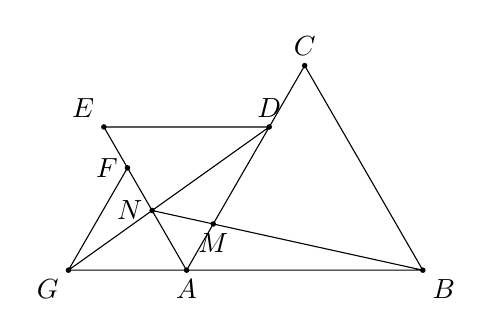
\begin{tikzpicture}[scale=1.5]
                \coordinate [label=below left:$G$] (G) at (0,0);
                \coordinate [label=left:$F$] (F) at (0.5,{sqrt(3)/2});
                \coordinate [label=below:$A$] (A) at (1,0);
                \coordinate [label=above:$C$] (C) at (2,{sqrt(3)});
                \coordinate [label=below right:$B$] (B) at (3,0);
                \coordinate [label=above left:$E$] (E) at (0.3,{0.7*sqrt(3)});
                \coordinate [label=above:$D$] (D) at (1.7,{0.7*sqrt(3)});
                \coordinate [label=left:$N$] (N) at (intersection of D--G and A--E);
                \coordinate [label=below:$M$] (M) at (intersection of B--N and A--C);
                \draw (F)--(G)--(A)--(B)--(C)--(A)--cycle (F)--(E)--(D) (B)--(N) (D)--(G);
                \foreach \point in {A,B,C,D,E,F,G,M,N}
                    \fill (\point) circle (1/1.5pt);
            \end{tikzpicture}\\
            {\kai (第\thekong 题图)}
        \end{center}
    \end{kong}

    \begin{kong}\rm
        已知正数$a,b,c$满足$a^2+ab+ac+bc=6+2\sqrt{5}$, 则$3a+b+2c$最小值是\hx{2}.
    \end{kong}

    \newpage

    {\bf \hei 二\dh 解答题}(共45分)

    \begin{kong}\rm
        {\kai (本题满分10分)}

        求所有的非零实数$k$, 使得关于$x$的方程$kx^2+(4k+1)x+3-k=0$的根都是整数.
    \end{kong}

    \vspace*{9cm}

    \begin{kong}\rm
        {\kai (本题满分10分)}

        证明:

        (1)若$x>0,y>0$, 则$\dfrac{x^2}{x+y}\geq\dfrac{3x-y}{4}$;

        (2)若$x,y,z>0$, 则$\dfrac{x^3}{x+y}+\dfrac{y^3}{y+z}+\dfrac{z^3}{z+x}\geq\dfrac{xy+yz+zx}{2}$.
    \end{kong}

    \newpage
    
    \begin{kong}\rm
        {\kai (本题满分12分)}

        (1)是否存在正整数$a,b$, 使得$a^2+2b,b^2+2a$都是完全平方数? 若存在, 求出所有满足条件的$a,b$, 若不存在, 请说明理由;

        (2)求不定方程$3^x+4^y=5^z$的所有正整数解$(x,y,z)$.
    \end{kong}

    \newpage

    \begin{kong}\rm
        {\kai (本题满分13分)}

        如图, 在$\triangle ABC$中, 点$E\tdh F$分别为边$AB\tdh AC$上两点, $BF$与$CE$交于点$D$, 连结$AD$, 与$EF$交于点$M$, $AD$的延长线与$BC$交于点$N$.

        (1)若$AE=EB,CF=2AF$, 求$\dfrac{AM}{MD}$与$\dfrac{AN}{DN}$的值;

        (2)若点$E\tdh F$分别为$AB\tdh AC$上任意两点时, 你能否猜出关于$\dfrac{AM}{MD}$与$\dfrac{AN}{DN}$的关系的一般结论, 并证明你的猜想.

        \begin{flushright}
            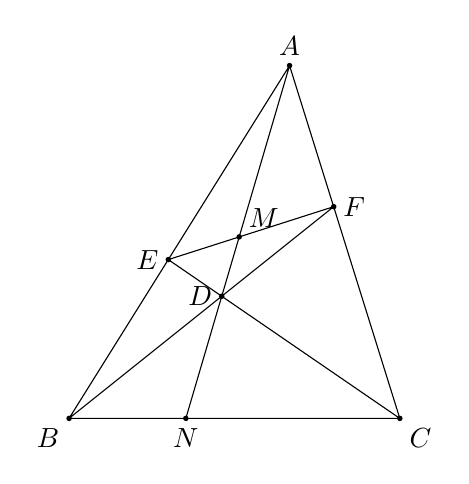
\begin{tikzpicture}[scale=1.4]
                \coordinate [label=below left:$B$] (B) at (0,0);
                \coordinate [label=below right:$C$] (C) at (3,0);
                \coordinate [label=above:$A$] (A) at (2,3.2);
                \coordinate [label=left:$E$] (E) at ($(B)!0.45!(A)$);
                \coordinate [label=right:$F$] (F) at ($(C)!0.6!(A)$);
                \coordinate [label=left:$D$] (D) at (intersection of B--F and C--E);
                \coordinate [label=above right:$M$] (M) at (intersection of E--F and A--D);
                \coordinate [label=below:$N$] (N) at (intersection of A--D and B--C);
                \draw (A)--(B)--(C)--cycle (B)--(F)--(E)--(C) (A)--(N);
                \foreach \point in {A,B,C,D,E,F,M,N}
                    \fill (\point) circle (1/1.4pt);
            \end{tikzpicture}\\
            {\kai (第\thekong 题图)\hspace*{1.65cm}}
        \end{flushright}
    \end{kong}
\end{document}